\documentclass[12pt]{article}
\usepackage{titling}
\usepackage{setspace}
\usepackage{hyperref}
\usepackage{graphicx}
\usepackage{lipsum}
\usepackage[margin=1in]{geometry}

\newcommand{\PutTitle}[1]
{
    \begin{center}
        {\huge\bfseries\thetitle}\\
        by \theauthor\\
        \thedate\\
        #1        
    \end{center}
    \hrule
    \vspace{2ex}
}

\setlength\paperwidth{8.5in}
\setlength\paperheight{11in}
\setlength\parindent{24pt}

\hypersetup
{
    colorlinks=true,
    linkcolor=blue,
    urlcolor=blue,
}

\begin{document}

\title{Sobre Cultura Semana 6}
\author{Jonah Mondragon}
\date{\today}
\PutTitle{Spanish El Periodo 8}

\doublespacing

La ubicación: Belice limita con Guatemala.

Aquí es una mapa de Belice:\\
\begin{center}
    \vspace{-4ex}
    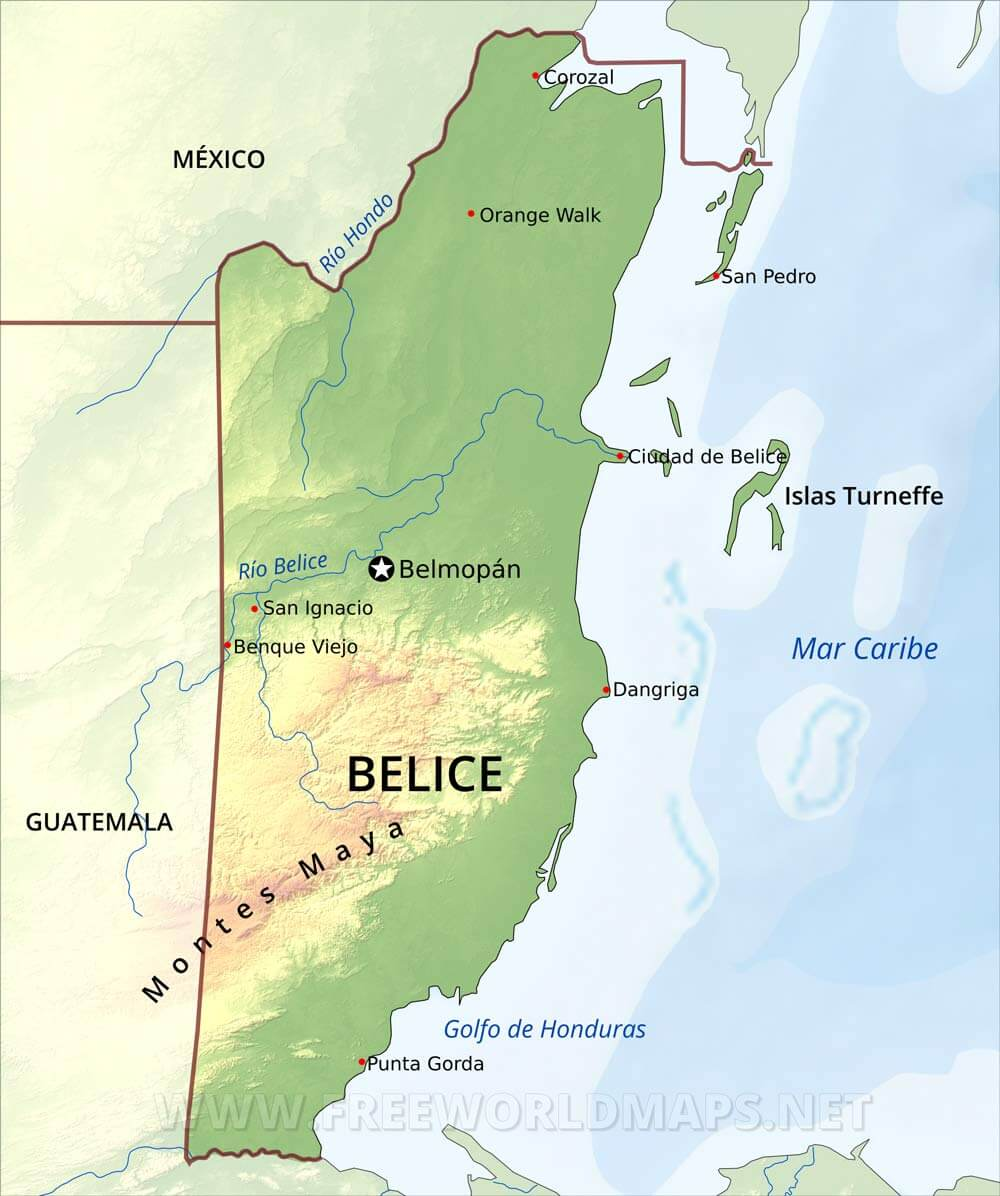
\includegraphics[width=4.25in,height=5.5in]{foto_de_Belice.jpg}
\end{center}

La capital de Belice es Belmopán

Otras ciudades importantes son San Pedro, Bella Vista, San Narciso y San José.

La población es trescientos noventa mil trescientos cincuenta y tres de habitantes.

Los idiomas hablados son inglés (la idioma oficial es inglés) y español.

La moneda oficial de Belice es el Dólar de Belice.

El presidente o presidenta de Belice es Dean Barrow.

Las comidas típicas de Belice son Sopa de pollo, Bundiga, Sopa Hadut y Tamales.

La música de......... es. 

Personajes importantes de .......... son..  Son conocidos por.......

Algo importante sobre........ es......

Include photos (fotos) otro cognado o dibujos.  

 

You may submit this work online or on paper. 

If you submit it on paper, make sure to type here " Lo hice en papel"

\end{document}

